\let\negmedspace\undefined
\let\negthickspace\undefined
\documentclass[journal]{IEEEtran}
\usepackage[a5paper, margin=10mm, onecolumn]{geometry}
%\usepackage{lmodern} % Ensure lmodern is loaded for pdflatex
\usepackage{tfrupee} % Include tfrupee package

\setlength{\headheight}{1cm} % Set the height of the header box
\setlength{\headsep}{0mm}     % Set the distance between the header box and the top of the text

\usepackage{gvv-book}
\usepackage{comment}
\usepackage{gvv}
\usepackage{cite}
\usepackage{amsmath,amssymb,amsfonts,amsthm}
\usepackage{algorithmic}
\usepackage{graphicx}
\usepackage{textcomp}
\usepackage{xcolor}
%\usepackage{txfonts}
\usepackage{listings}
\usepackage{enumitem}
\usepackage{mathtools}
\usepackage{gensymb}
\usepackage{comment}
\usepackage[breaklinks=true]{hyperref}
\usepackage{tkz-euclide} 
\usepackage{listings}
% \usepackage{gvv}                                        
\def\inputGnumericTable{}                                 
\usepackage[latin1]{inputenc}                                
\usepackage{color}                                            
\usepackage{array}                                            
\usepackage{longtable}                                       
\usepackage{calc}                                             
\usepackage{multirow}                                         
\usepackage{hhline}                                           
\usepackage{ifthen}                                           
\usepackage{lscape}
\usepackage{circuitikz}
\tikzstyle{block} = [rectangle, draw, fill=blue!20, 
    text width=4em, text centered, rounded corners, minimum height=3em]
\tikzstyle{sum} = [draw, fill=blue!10, circle, minimum size=1cm, node distance=1.5cm]
\tikzstyle{input} = [coordinate]
\tikzstyle{output} = [coordinate]


\begin{document}

\bibliographystyle{IEEEtran}
\vspace{3cm}

\title{8.4.16}
\author{EE25BTECH11013 - Bhargav}
\maketitle
    {\let\newpage\relax\maketitle}

\renewcommand{\thefigure}{\theenumi}
\renewcommand{\thetable}{\theenumi}
\setlength{\intextsep}{10pt} % Space between text and floats

\numberwithin{equation}{enumi}
\numberwithin{figure}{enumi}
\renewcommand{\thetable}{\theenumi}

\textbf{Question}: \\
Let the eccentricity of the hyperbola $\frac{x^2}{a^2}-\frac{y^2}{b^2}=1$ be reciprocal to that of the ellipse $x^2+4y^2=4$. If the hyperbola
passes through a focus of the ellipse, then 

\begin{enumerate}
	\item the equation of the hyperbola is $\frac{x^2}{3}-\frac{y^2}{2}=1$
	\item a focus of the hyperbola is $(2,0)$
	\item the eccentricity of the hyperbola is $\sqrt{\frac{5}{3}}$
	\item the equation of the hyperbola is $x^2-3y^2=3$
\end{enumerate}
\solution \\
The general equation of the conic can be written as:
\begin{align}
\vec{x^T}\vec{V}\vec{x} + 2\vec{u^T}\vec{x} + f = 0
\end{align}
For the given ellipse, we get
\begin{align}
\vec{V} = \myvec{\frac{1}{4} & 0 \\ 0 & 1}, f = -1, \vec{u} = \myvec{0 \\ 0}
\end{align}
Since the major axis of the ellipse is X-axis, $\vec{n} = \myvec{1 \\ 0}$ \\
Using the formula:
\begin{align}
\vec{V} = \norm{n}^2\vec{I} - e^2\vec{n}\vec{n^T}
\end{align}
For both ellipse and hyperbola, we get:
\begin{align}
\vec{V} = \myvec{1-e^2 & 0 \\ 0 & 1}
\end{align}
Comparing with $\vec{V}$ obtained for an ellipse, we get $e_E = \frac{\sqrt{3}}{2}$

Given that $e_H\cdot e_E = 1$\\
Thus, the eccentricity of the hyperbola is $e_H = \frac{2}{\sqrt{3}}$\\

Substituting $e_H=\frac{2}{\sqrt{3}}$ in the hyperbola equation, (f=1) 
\begin{align}
\vec{x^T}\myvec{-\frac{1}{3} & 0 \\ 0 & 1}\vec{x} + 1 = 0 \implies \frac{x^2}{3} - y^2 = 1
\end{align}
To find the focal length of the hyperbola, we use:
\begin{align}
c = \sqrt{\frac{\abs{\lambda_1 - \lambda_2}}{\norm{\vec{V}}}}
\end{align}
The eigenvalues of a diagonal matrix are the diagonal elements of matrix $\vec{V}$ for the hyperbola
\begin{align}
\lambda_1 = -\frac{1}{3} , \lambda_2 = 1
\end{align}

\begin{align}
\implies c = 2
\end{align}
Thus, the focus of the hyperbola is $\myvec{\pm 2 \\ 0}$

Option (2) and (4) are correct

The theoretical solution can be verified graphically

\begin{figure}[H]
    \centering
    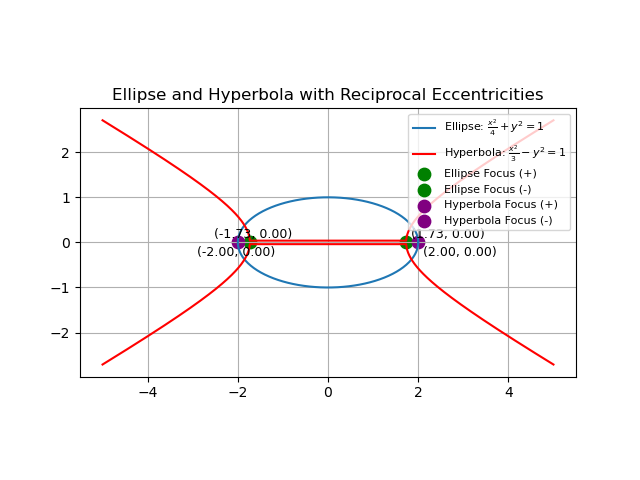
\includegraphics[height=0.5\textheight, keepaspectratio]{figs/Figure_1.png}
    \label{figure_1}
\end{figure}

\end{document}



